\section*{Exercise 5.13}
We do this exercise with unstandardized residuals. The solution and intuition is similar for the other residuals, but requires more calculations to find the theoretical residual lines.
\begin{lstlisting}[language=R]
# Parameters for the problem.

n = 100
min = 0
max = 100

# Make the theoretical residuals.

x = seq(min, max, by = 0.1)
y = plogis(-2.0 + 0.04 * x)

plot(
  x = x, 
  y = -y, 
  type = "l", 
  ylim = c(-1, 1), 
  main = "Residuals",
  ylab = "Residuals")

lines(x = x, y = 1 - y)

# Simulate some values.

set.seed(313) # Reproducibility.
x = runif(n = n, min = min, max = max)
y = -2.0 + 0.04 * x + rlogis(n) >= 0
model = glm(y ~ x, family = binomial(link = "logit"))

# Add to plot.
col = c("red", "blue")[y + 1]
points(x, y - fitted(model), col = col, pch = 20)
\end{lstlisting}

\begin{center}
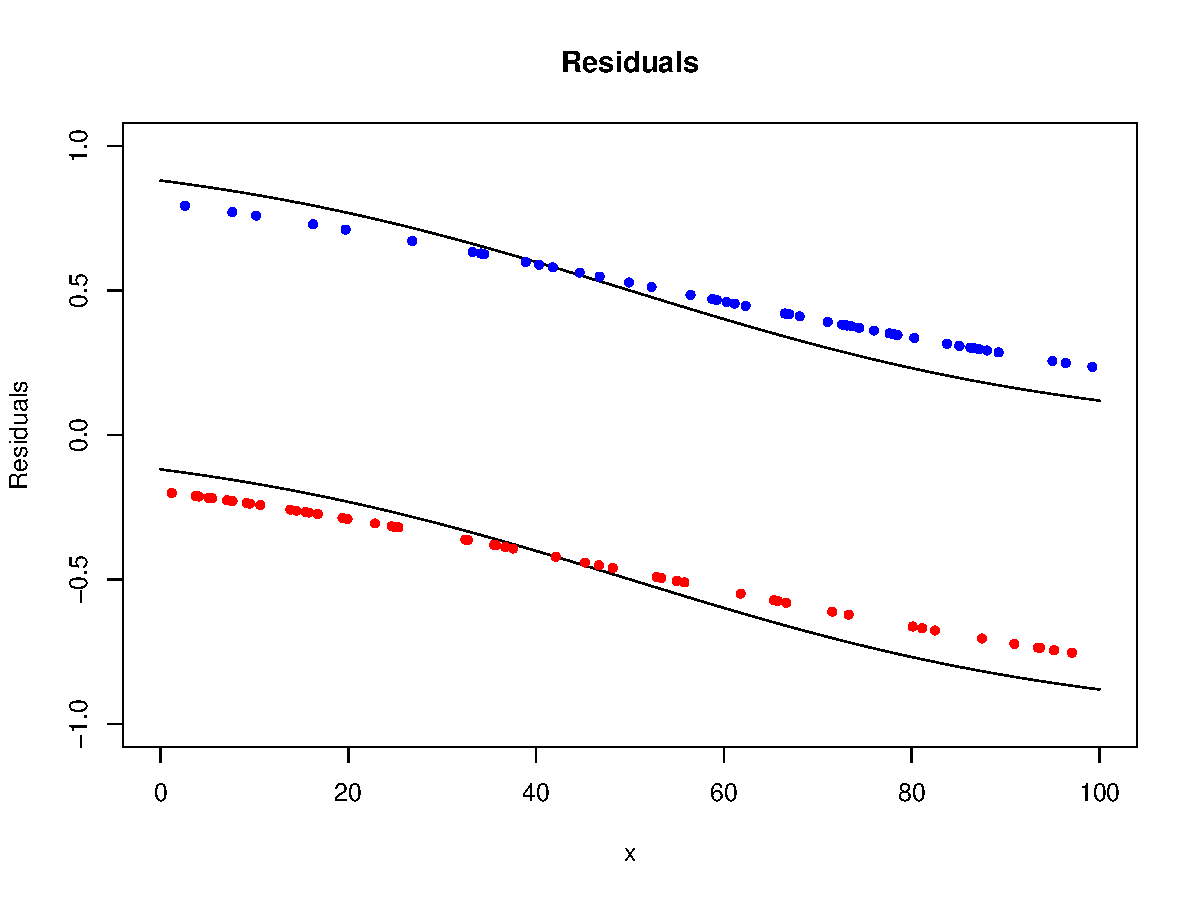
\includegraphics[scale=0.7]{figures/exercise-5.13.pdf}
\end{center}